\scanpage{43}

\uline{de \(n\)}. En effet, on a
\[
\varphi_X(E(n))=\varphi_X(E)\deleted{\unsure{\varphi}}e^{n\xi}.
\]
d'où
\[
\tau_h(X)\varphi_X(E(n))=\underbrace{\tau_h(X)\varphi_X(E)}e^{n\xi}=\sum_k n^k\left[\frac{\xi^k}{k!}\tau_h(X)\varphi_X(E)\right]
\]
et
\[
f_*(\tau_h(X)\varphi_X(E(n))=\sum_k n^k f_*\left(\frac{\xi^k}{k!}\tau_h(X)\varphi_X(E)\right)
\]

\figure{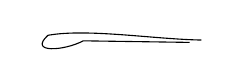
\begin{tikzpicture}[x=1cm,y=1cm]\draw (0,0)..controls (-.25,-.23) and (.2,-.2)..(.45,-.07)--(1.8,-.09);\draw (0,0)..controls (.5,.09) and (1.35,-.05)..(1.95,-.06);\end{tikzpicture}}

Cas de morphisme propre quelconque.

1) Morphisme d'une courbe \deleted{\(\unsure{Y}\)} \inserted{\unsure{nons. complète|irr. complète}} \(X\) dans une variété \(X\).

On peut évidemment supposer \(f\) non constant, \(X\) et \(Y\) irréductibles.

\deleted{\unsure{X et Y irréductibles}}

On a \(K(\unsure{X})\simeq\mathbb Z+\mathfrak P(\unsure{X})\), \unsure{un} l'isomorphisme étant précisément donné par la application \deleted{\(\unsure{C}\)}\(\widetilde C\) de Chern. On doit donc \deleted{\unsure{définir}}\inserted{calculer}, pour \(\xi=(n,d)\) son image \(f_!(\xi)\in K(Y)\) en fonction de \(n,d\). Noter que \(\varphi_X(\xi)=n+\underline d\), \(\widetilde C(T_X)=(1,-\underline k)\) donc \(\tau_h(X)=\frac{-\underline k}{1-e^{\underline k}}=\unsure{1-\tfrac12\underline k|1\,\tfrac12\underline k}\), \(\underline k\) étant la classe canonique. Donc

\deleted{a) \(X\) est courbe (non singulière irréductible).}
\[
\varphi_X(\xi)\tau_h(\unsure{X})=(1-\tfrac12\underline k)(n+\underline d)=\deleted{\unsure{n+\underline d+\underline k}}n+(\underline d-n\tfrac12\underline k)
\]

 a) \(Y\) est une courbe. Soit \(\underline{k'}\) son diviseur canonique d'où \(\tau_h(Y)=1-\tfrac12\underline{k'}\). Soit \(\delta\) le \uline{degré} de \(f\).

alors on a \(f_*(1)=\delta\), donc
\[
f_*(\varphi_X(\xi)\tau_h(X))=n\delta+\left(f_*(\underline d)-nf_*(\tfrac12\underline k)\right)
\]
d'où
\[
\begin{aligned}
\varphi_X(f_!(\xi))&=\tau_h(Y)^{-1}f_*(\mathord{\cdot}\mathbin{\text{---}})=(1+\tfrac12\underline{k'})(n\delta+(f_*(\underline d)-nf_*(\tfrac12\underline k)))\\
&=n\delta+\left[n\delta\tfrac12\underline{k'}+f_*(\underline d)-nf_*(\tfrac12\underline k)\right]
\end{aligned}
\]
par suite
\[
\boxed{f_!(\xi)=\left(n\delta,\ n\delta\tfrac12\underline{k}_Y+f_*(\underline d)-nf_*(\tfrac12\underline{k}_X)\right)}\qquad(f:x\longrightarrow Y)
\]

\margin{R}
\figure{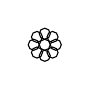
\begin{tikzpicture}[scale=.2]\draw (0,0) circle (.35);\foreach \a in {0,45,...,315}{\draw (\a:.7) circle (.35);}\end{tikzpicture}}
\margin{ARGENTINA LINEN TYPEWRITER}
\figure{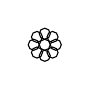
\begin{tikzpicture}[scale=.2]\draw (0,0) circle (.35);\foreach \a in {0,45,...,315}{\draw (\a:.7) circle (.35);}\end{tikzpicture}}
\margin{A}
\margin{42}
